% Options for packages loaded elsewhere
\PassOptionsToPackage{unicode}{hyperref}
\PassOptionsToPackage{hyphens}{url}
%
\documentclass[
]{article}
\usepackage{lmodern}
\usepackage{amssymb,amsmath}
\usepackage{ifxetex,ifluatex}
\ifnum 0\ifxetex 1\fi\ifluatex 1\fi=0 % if pdftex
  \usepackage[T1]{fontenc}
  \usepackage[utf8]{inputenc}
  \usepackage{textcomp} % provide euro and other symbols
\else % if luatex or xetex
  \usepackage{unicode-math}
  \defaultfontfeatures{Scale=MatchLowercase}
  \defaultfontfeatures[\rmfamily]{Ligatures=TeX,Scale=1}
\fi
% Use upquote if available, for straight quotes in verbatim environments
\IfFileExists{upquote.sty}{\usepackage{upquote}}{}
\IfFileExists{microtype.sty}{% use microtype if available
  \usepackage[]{microtype}
  \UseMicrotypeSet[protrusion]{basicmath} % disable protrusion for tt fonts
}{}
\usepackage{xcolor}
\IfFileExists{xurl.sty}{\usepackage{xurl}}{} % add URL line breaks if available
\IfFileExists{bookmark.sty}{\usepackage{bookmark}}{\usepackage{hyperref}}
\hypersetup{
  pdftitle={Supplementary analyses for `Word structure in early Quechua speech'},
  hidelinks,
  pdfcreator={LaTeX via pandoc}}
\urlstyle{same} % disable monospaced font for URLs
\usepackage[margin=1in]{geometry}
\usepackage{longtable,booktabs}
% Correct order of tables after \paragraph or \subparagraph
\usepackage{etoolbox}
\makeatletter
\patchcmd\longtable{\par}{\if@noskipsec\mbox{}\fi\par}{}{}
\makeatother
% Allow footnotes in longtable head/foot
\IfFileExists{footnotehyper.sty}{\usepackage{footnotehyper}}{\usepackage{footnote}}
\makesavenoteenv{longtable}
\usepackage{graphicx,grffile}
\makeatletter
\def\maxwidth{\ifdim\Gin@nat@width>\linewidth\linewidth\else\Gin@nat@width\fi}
\def\maxheight{\ifdim\Gin@nat@height>\textheight\textheight\else\Gin@nat@height\fi}
\makeatother
% Scale images if necessary, so that they will not overflow the page
% margins by default, and it is still possible to overwrite the defaults
% using explicit options in \includegraphics[width, height, ...]{}
\setkeys{Gin}{width=\maxwidth,height=\maxheight,keepaspectratio}
% Set default figure placement to htbp
\makeatletter
\def\fps@figure{htbp}
\makeatother
\setlength{\emergencystretch}{3em} % prevent overfull lines
\providecommand{\tightlist}{%
  \setlength{\itemsep}{0pt}\setlength{\parskip}{0pt}}
\setcounter{secnumdepth}{5}
\usepackage{booktabs}
\usepackage{longtable}
\usepackage{array}
\usepackage{multirow}
\usepackage{wrapfig}
\usepackage{float}
\usepackage{colortbl}
\usepackage{pdflscape}
\usepackage{tabu}
\usepackage{threeparttable}
\usepackage{threeparttablex}
\usepackage[normalem]{ulem}
\usepackage{makecell}
\usepackage{xcolor}

\title{Supplementary analyses for
`Word structure in early Quechua speech'}
\author{}
\date{\vspace{-2.5em}}

\begin{document}
\maketitle

{
\setcounter{tocdepth}{2}
\tableofcontents
}
\hypertarget{results}{%
\section{Results}\label{results}}

The primary research objective of this study is to measure the speech production patterns of child and adult Quechua speakers between and within morphemes. Results begin with descriptive statistics concerning the amount of coarticulation and VC sequence duration by age group and morphological environment (within versus between morphemes). Then, a series of models are fit to predict coarticulation and duration by age and morphological environment. These models are complemented by an analysis highlighting how coarticulation interacts with duration differently in adults and children in the two morphological environments.

All analyses were conducted in the RStudio computing environment (version: 1.3.1056; rstudio, 2020). Data visualizations were created with \texttt{ggplot2} (Wickham, 2016). Modeling was conducted using the \texttt{lme4} (Bates et al., 2015), \texttt{lmerTest} (Kuznetsova et al., 2017), and \texttt{glmmTMB} (Brooks et al., 2017) packages and summaries were presented with \texttt{papaja} (Aust \& Barth, 2019) and \texttt{Stargazer} (Hlavac, 2018). Tests of residual normality were conducted using the \texttt{normtest} package (Gavrilov \& Pusev, 2014). The significance of potential model parameters was determined using a combination of log-likelihood comparisons between models, AIC estimations, and p-values procured from model summaries. In all models, continuous predictors were mean-centered to facilitate model interpretation.

\hypertarget{modeling-interaction-of-coarticulation-and-duration}{%
\subsection{Modeling interaction of coarticulation and duration}\label{modeling-interaction-of-coarticulation-and-duration}}

A series of linear mixed effect models were fit to predict degree of coarticulation (Mel spectral distance between each V and C). The residual \textbf{Sequence duration} is limited to non-negative values (all VC sequences had a duration), with a resultant right skew to the data distribution.\footnote{Shapiro tests of kurtosis and skewness for \textbf{Sequence duration} indicated that we could reject the null hypothesis that the residual's distribution did not differ significantly from a normal distribution. Kurtosis t=5.53, p\textless.001 and skewness: t=1.07, p\textless.001 (Shapiro et al., 1968).} Consequently, \textbf{Sequence duration} was log-normalized prior to model fitting.

Baseline models included random slopes of \textbf{Participant} by \textbf{Word}. Model building then began in a forward-testing manner with predictors added in the following order: \textbf{Syllable Count} (fit with weighted effect coding for all models), \textbf{Sequence duration}, \textbf{VC sequence} ({[}ap{]} or {[}am{]}), \textbf{Age} (adult or child), \textbf{Environment} ({[}within morpheme or between morphemes{]}), and interactions. \textbf{Syllable Count} was included in the modeling in an attempt to isolate the effect of \textbf{Environment} on speech production from prosodic structure since within-morpheme stimulus items tended to be shorter than across-morpheme items (see Methods).

The best model fit included \textbf{Syllable Count} and the four-variable interaction of \textbf{Sequence duration}, \textbf{VC sequence}, \textbf{Age}, and \textbf{Environment}. The summary for the model containing adults and children together is included in Appendix A. This four-variable interaction indicates that the relationship between coarticulation and duration differs between adults and children. Given the difficulty in interpreting four-variable interactions, separate models were fit for adults and children to facilitate coefficient interpretation.

Best model fit for the adult and child models included \textbf{Syllable Count} and the three-variable interaction of \textbf{Sequence duration}, \textbf{VC sequence}, and \textbf{Environment}. The final adult model summary is listed in Table 1 and the child model summary is listed in Table 2.\footnote{In the model summaries for the children and adults, the coefficients and standard error measurements were multiplied by 100 to make the otherwise small coefficients more interpretable. This step does not effect the direction or magnitude of the effect between predictors and outcome variables.}

For the child model, the addition of the variable \textbf{Age Group} (levels: 5, 6, 7, 8, 9, 10; fit with weighted effect coding) improved upon a model with \textbf{Syllable Count} and the interaction of \textbf{Sequence duration}, \textbf{VC sequence}, and \textbf{Environment}. This significance of \textbf{Age Group} indicates that the child participants tended to coarticulate more with age, just as the adults studied coarticulated more than the children, likely because the older children and adults spoke faster.

\begin{table}[!htbp] \centering 
  \caption{Model predicting coarticulation in adults} 
  \label{} 
\begin{tabular}{@{\extracolsep{5pt}}lc} 
\\[-1.8ex]\hline 
\hline \\[-1.8ex] 
 Intercept & 1.27 \\ 
  & ($-$5.40, 7.95) \\ 
  & \\ 
 Syllable count:2 & 2.74$^{***}$ \\ 
  & (0.80, 4.68) \\ 
  & \\ 
 Syllable count:3 & $-$0.88$^{**}$ \\ 
  & ($-$1.59, $-$0.17) \\ 
  & \\ 
 Syllable count:4 & $-$0.19 \\ 
  & ($-$1.52, 1.14) \\ 
  & \\ 
 Sequence duration & 2.01$^{**}$ \\ 
  & (0.09, 3.92) \\ 
  & \\ 
 Environment:across morpheme & 7.77$^{*}$ \\ 
  & ($-$0.40, 15.93) \\ 
  & \\ 
 VC sequence:[ap] & 13.64$^{***}$ \\ 
  & (6.04, 21.23) \\ 
  & \\ 
 Sequence duration*Environment:across morpheme & $-$2.11 \\ 
  & ($-$4.66, 0.43) \\ 
  & \\ 
 Sequence duration:VC sequence:[ap] & $-$2.08$^{*}$ \\ 
  & ($-$4.27, 0.11) \\ 
  & \\ 
 Environment:across morpheme*VC sequence:[ap] & $-$5.95 \\ 
  & ($-$15.03, 3.13) \\ 
  & \\ 
 Sequence duration*Environment:across morpheme*VC sequence:[ap] & 2.63$^{*}$ \\ 
  & ($-$0.20, 5.45) \\ 
  & \\ 
\hline \\[-1.8ex] 
Observations & 201 \\ 
Log Likelihood & $-$525.41 \\ 
Akaike Inf. Crit. & 1,076.82 \\ 
Bayesian Inf. Crit. & 1,119.77 \\ 
\hline 
\hline \\[-1.8ex] 
\textit{Note:}  & \multicolumn{1}{r}{$^{*}$p$<$0.1; $^{**}$p$<$0.05; $^{***}$p$<$0.01} \\ 
\end{tabular} 
\end{table}

\begin{table}[!htbp] \centering 
  \caption{Model predicting coarticulation in children} 
  \label{} 
\begin{tabular}{@{\extracolsep{5pt}}lc} 
\\[-1.8ex]\hline 
\hline \\[-1.8ex] 
 Intercept & 8.01$^{***}$ \\ 
  & (6.61, 9.42) \\ 
  & \\ 
 Syllable count:2 & 0.62 \\ 
  & ($-$0.30, 1.54) \\ 
  & \\ 
 Syllable count:3 & $-$0.17 \\ 
  & ($-$0.67, 0.33) \\ 
  & \\ 
 Syllable count:4 & $-$0.11 \\ 
  & ($-$0.84, 0.62) \\ 
  & \\ 
 Sequence duration & 0.22 \\ 
  & ($-$0.15, 0.58) \\ 
  & \\ 
 Environment:across morpheme & 0.57 \\ 
  & ($-$1.69, 2.82) \\ 
  & \\ 
 VC sequence:[ap] & 8.65$^{***}$ \\ 
  & (5.85, 11.46) \\ 
  & \\ 
 Age:6 & 0.53$^{**}$ \\ 
  & (0.06, 0.99) \\ 
  & \\ 
 Age:7 & 0.07 \\ 
  & ($-$0.34, 0.48) \\ 
  & \\ 
 Age:8 & 2.06$^{***}$ \\ 
  & (1.50, 2.61) \\ 
  & \\ 
 Age:9 & $-$1.83$^{***}$ \\ 
  & ($-$2.66, $-$1.00) \\ 
  & \\ 
 Age:10 & $-$2.26$^{***}$ \\ 
  & ($-$3.08, $-$1.44) \\ 
  & \\ 
 Sequence duration*Environment:across morpheme & $-$0.03 \\ 
  & ($-$0.65, 0.58) \\ 
  & \\ 
 Sequence duration:VC sequence:[ap] & 0.24 \\ 
  & ($-$0.40, 0.89) \\ 
  & \\ 
 Environment:across morpheme*VC sequence:[ap] & 0.68 \\ 
  & ($-$2.76, 4.12) \\ 
  & \\ 
 Sequence duration*Environment:across morpheme*VC sequence:[ap] & $-$0.77$^{*}$ \\ 
  & ($-$1.64, 0.10) \\ 
  & \\ 
\hline \\[-1.8ex] 
Observations & 2,004 \\ 
Log Likelihood & $-$5,786.85 \\ 
Akaike Inf. Crit. & 11,609.71 \\ 
Bayesian Inf. Crit. & 11,710.56 \\ 
\hline 
\hline \\[-1.8ex] 
\textit{Note:}  & \multicolumn{1}{r}{$^{*}$p$<$0.1; $^{**}$p$<$0.05; $^{***}$p$<$0.01} \\ 
\end{tabular} 
\end{table}

In the adult and child models, a positive coefficient for the predictor \textbf{VC sequence}, with the reference level `{[}am{]}', shows that there was greater spectral distance between the segments in {[}ap{]} than {[}am{]}, as we would anticipate given the acoustic signatures of {[}m{]} (voiced, sonorant) versus {[}p{]} (voiceless, transient).

A positive coefficient for \textbf{Sequence duration} indicates that longer duration VC sequences tend to be less coarticulated (greater spectral distance between phones). There is, however, an interaction between several of these predictors, which will demonstrate that children in particular do not always coarticulate less in longer-duration sequences. The direction of the interaction between \textbf{Sequence duration}, \textbf{VC sequence}, and \textbf{Environment} differs between the adult and child speakers so this will be interpreted separately for the two groups in the following section.

Finally, the parameter \textbf{Syllable Count} was significant for the adult and child models. However, the direction of the effect differed. Children tended to coarticulate progressively more in longer words. Adults coarticulated differently by word size, but coarticulation did not increase in longer words.

~
~

\begin{figure}
\centering
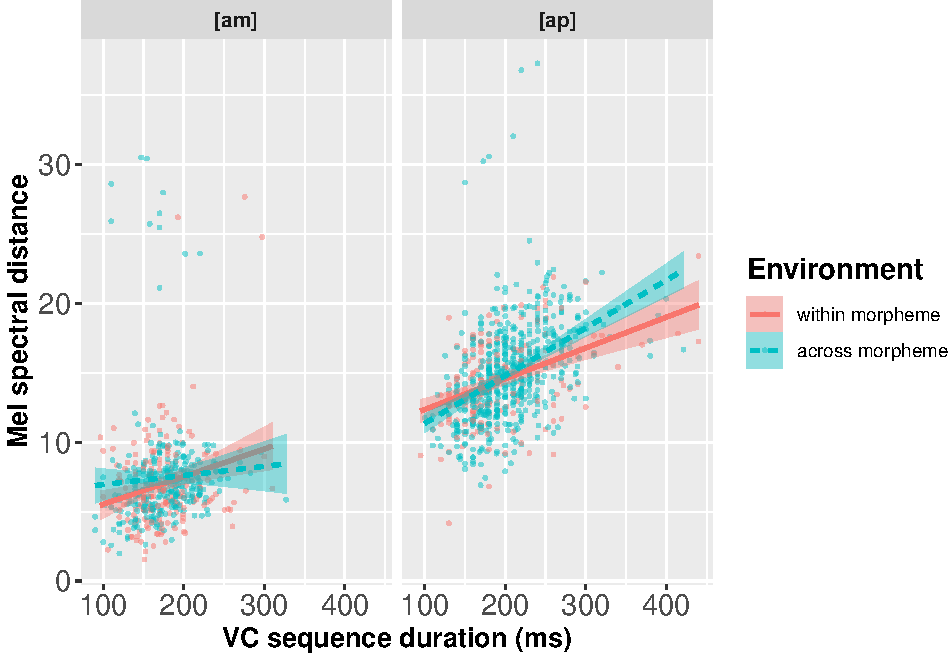
\includegraphics{supp_analysis_files/figure-latex/adult-int-plot-1.pdf}
\caption{\label{fig:adult-int-plot}Coarticulation within VC sequence by sequence duration and morphological environment in adult speakers}
\end{figure}

\begin{figure}
\centering
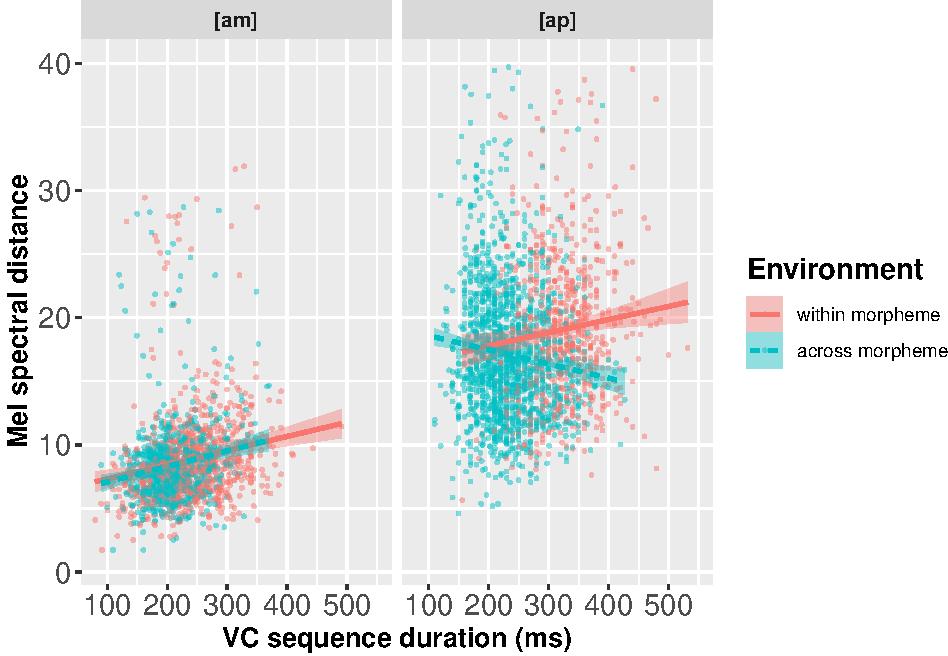
\includegraphics{supp_analysis_files/figure-latex/child-int-plot-1.pdf}
\caption{\label{fig:child-int-plot}Coarticulation within VC sequence by sequence duration and morphological environment in all child speakers}
\end{figure}

\hypertarget{adults}{%
\paragraph{Adults}\label{adults}}

For the adult model, the interaction between \textbf{Sequence duration}, \textbf{VC sequence}, and \textbf{Environment} suggests a difference in the relationship between the response variable---amount of coarticulation---and \textbf{Sequence duration} that differs by \textbf{Environment} and \textbf{VC sequence} (note that this interaction only approaches significance {[}p\textless.10{]} in these linear models). As Figure \ref{fig:adult-int-plot} demonstrates, this difference by \textbf{Environment} is apparent in the steepness of the slope for the `across morpheme' and `within morpheme' conditions for {[}am{]} and {[}ap{]}. To quantify this difference for the sequence {[}am{]}, the slopes of the two conditions were calculated. As the {[}am{]} panel in Figure \ref{fig:adult-int-plot} suggests, the slope for the `within morpheme' condition was steeper (2.14) than the slope for the `across morpheme' condition (2.06),\footnote{To reflect the data visualizations, these slopes were calculated on the beta coefficients before the coefficients were scaled by 100.} suggesting a different relationship between duration and articulation between the two word environments in adults.

Overall, the interaction \textbf{Sequence duration}, \textbf{VC sequence}, and \textbf{Environment} in adult speakers shows two important results: first, adults distinguish by word environment, both for {[}ap{]} versus {[}a\#p{]} sequences and {[}am{]} versus {[}a\#m{]} sequences. Second, complicating this finding, is the fact that adults distinguish between word environments differently depending upon the VC sequence. For {[}ap{]}, though adults coarticulate roughly equally across and within morphemes, the relationship between duration and coarticulation (longer duration equates to less coarticulation) is stronger in the `across morpheme' condition. For {[}am{]}, adults also distinguish between the two morphological environments by the relationship of VC duration and coarticulatory degree, but the effect of condition is reversed: the relationship between duration and coarticulation is stronger for the `within morpheme' condition.

Thus, returning to one of the central research questions - does adult coarticulation differ by word environment - we find that adults do coarticulate differently in the two word environments. Despite the differences by word environment, there was still a positive relationship between duration and amount of coarticulation for all combinations of VC sequences and word environments. Adults consistently coarticulate less in longer-duration sequences. This result suggests that adult speakers may have one overarching articulatory plan for all environments and both VC sequences measured. The following section demonstrates how this relationship between duration and coarticulation may not be uniform between adults and children.

\hypertarget{children}{%
\paragraph{Children}\label{children}}

In the child model, the significant interaction of \textbf{Sequence duration}, \textbf{VC sequence}, and \textbf{Environment} suggests that children do not coarticulate similarly in longer-duration sequences for all combinations of \textbf{Environment} and \textbf{VC sequence} (Figure \ref{fig:child-int-plot}). Specifically, for {[}ap{]} sequences that occur across morpheme boundaries, the negative slope indicates that children actually coarticulate \emph{more} in longer duration sequences. The positive slope for the within morpheme boundary condition suggests that children coarticulate less in longer-duration sequences, in line with all of the adult patterns. So, children coarticulate more between segments at morpheme boundaries in words inflected with the locative marker \emph{-pi} than between those same segments that occur within morphemes.

\begin{figure}
\centering
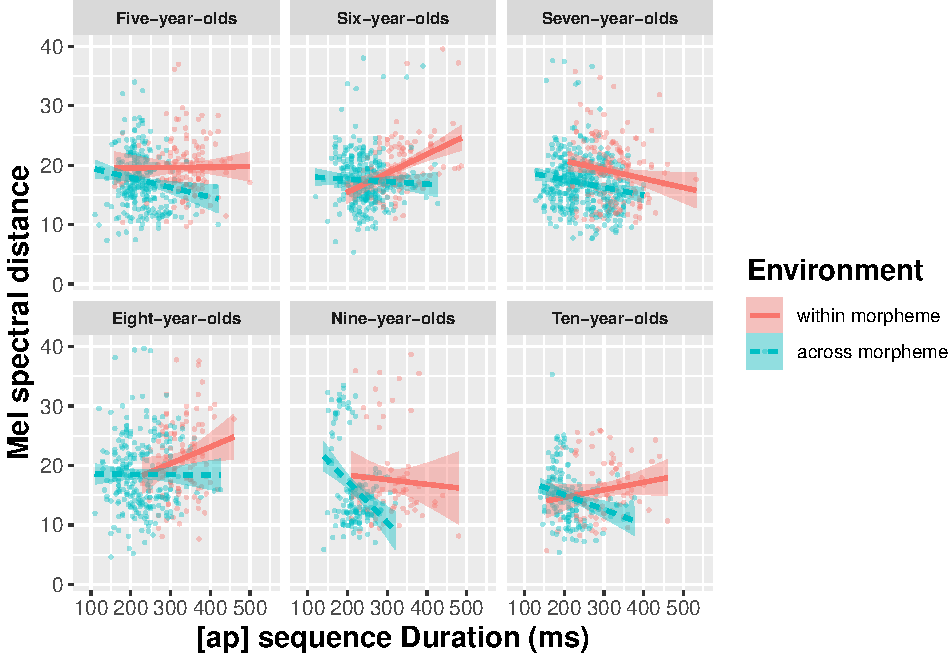
\includegraphics{supp_analysis_files/figure-latex/child-facet-ap-1.pdf}
\caption{\label{fig:child-facet-ap}Coarticulation within {[}ap{]} by sequence duration, morphological environment, and age in child speakers}
\end{figure}

This negative relationship between duration and spectral distance is counter to the positive relationship for every combination of VC sequence and word environment in adult speakers. Adults consistently coarticulate less in longer-duration sequences regardless of environment or VC sequence. The facet plot in Figure \ref{fig:child-facet-ap} plots this relationship between duration and coarticulation for {[}ap{]} for each age group (5-10 years) to ensure a consistent pattern. All age groups show the same negative relationship: the longer the {[}ap{]} sequence, the more the children coarticulate between {[}a{]} and {[}p{]} in the across morpheme condition.

\begin{figure}
\centering
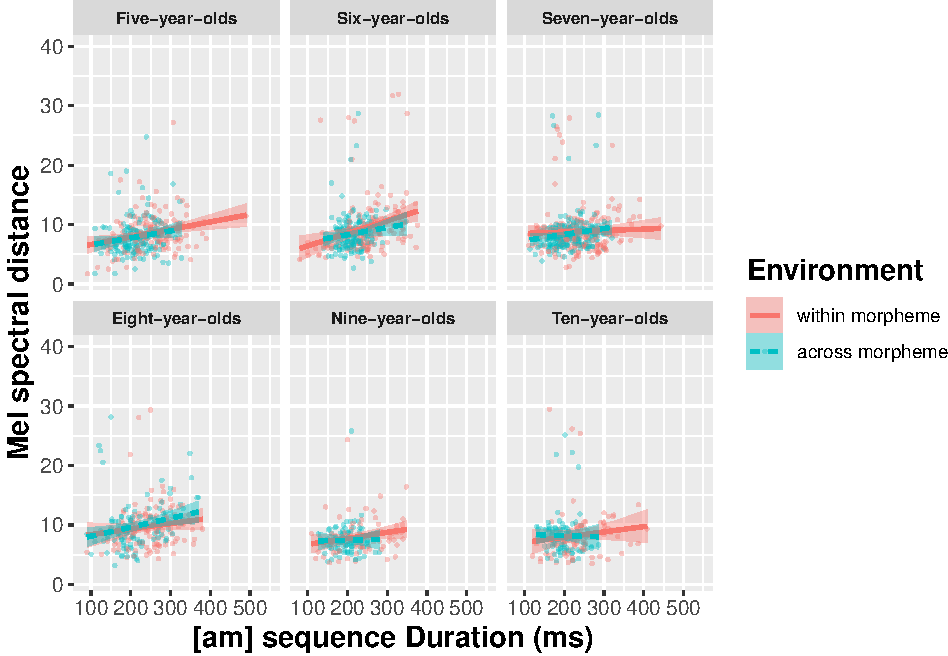
\includegraphics{supp_analysis_files/figure-latex/child-facet-am-1.pdf}
\caption{\label{fig:child-facet-am}Coarticulation within {[}am{]} by sequence duration, morphological environment, and age in child speakers}
\end{figure}

The results for {[}am{]} in children demonstrate broadly similar results to the adult speakers: children coarticulate less between segments in longer-duration {[}am{]} sequences. The facet plot in Figure \ref{fig:child-facet-am} once again shows a similar effect for each age group. Given the between-subject variability that typically characterizes child speech, these patterns by environment are further broken apart by individual child for each age group (age 5-10) in the manuscript to ensure no large outliers with regards to the patterning by word environment. The results by are broadly similar across speakers.

In sum, modeling results suggest that morphological structure is reflected in the speech of adults and children. However, the structure manifests in different ways between the two groups. Adults have a single plan for both environments, and even both VC sequences: adults coarticulate less in longer-duration sequences. For the most part, children show a similar duration-coarticulation relationship. The stark difference between adults and children emerges in the {[}ap{]} sequence patterning. Children differentiate between morphological environments via the relationship between duration and coarticulation as they coarticulate more in longer-duration sequences across morpheme boundaries and coarticulate \emph{less} in longer-duration sequences within morphemes. For words inflected with \emph{-man}, children show a similar pattern to adults, though children do not differentiate by environment coarticulatorily. Rather, across morpheme sequences are shorter in duration than within morpheme sequences for the children.

\hypertarget{appendices}{%
\section{Appendices}\label{appendices}}

\hypertarget{appendix-a}{%
\subsection{Appendix A}\label{appendix-a}}

\begin{table}[!htbp] \centering 
  \caption{Model predicting coarticulation in adults and children} 
  \label{} 
\begin{tabular}{@{\extracolsep{5pt}}lc} 
\\[-1.8ex]\hline 
\hline \\[-1.8ex] 
 Intercept & 4.28 \\ 
  & ($-$4.01, 12.57) \\ 
  & \\ 
 Syllable count:2 & 0.83$^{*}$ \\ 
  & ($-$0.05, 1.71) \\ 
  & \\ 
 Syllable count:3 & $-$0.28 \\ 
  & ($-$0.72, 0.17) \\ 
  & \\ 
 Syllable count:4 & $-$0.05 \\ 
  & ($-$0.73, 0.63) \\ 
  & \\ 
 Sequence duration & 1.82 \\ 
  & ($-$0.54, 4.17) \\ 
  & \\ 
 VC sequence:[ap] & 11.76$^{**}$ \\ 
  & (2.27, 21.24) \\ 
  & \\ 
 Age:child & 3.61 \\ 
  & ($-$4.77, 11.99) \\ 
  & \\ 
 Environment:across morpheme & 4.07 \\ 
  & ($-$6.14, 14.28) \\ 
  & \\ 
 Sequence duration:VC sequence:[ap] & $-$1.91 \\ 
  & ($-$4.59, 0.76) \\ 
  & \\ 
 Sequence duration:Age:child & $-$1.59 \\ 
  & ($-$3.97, 0.80) \\ 
  & \\ 
 VC sequence:[ap]*Age:child & $-$3.77 \\ 
  & ($-$13.67, 6.12) \\ 
  & \\ 
 Sequence duration*Environment:across morpheme & $-$1.85 \\ 
  & ($-$5.08, 1.38) \\ 
  & \\ 
 VC sequence:[ap]*Environment:across morpheme & $-$3.57 \\ 
  & ($-$15.02, 7.88) \\ 
  & \\ 
 Age:child*Environment:across morpheme & $-$4.03 \\ 
  & ($-$14.42, 6.36) \\ 
  & \\ 
 Sequence duration*VC sequence:[ap]*Age:child & 2.28 \\ 
  & ($-$0.47, 5.03) \\ 
  & \\ 
 Sequence duration*VC sequence:[ap]*Environment:across morpheme & 2.26 \\ 
  & ($-$1.29, 5.80) \\ 
  & \\ 
 Sequence duration*Age:child*Environment:across morpheme & 2.11 \\ 
  & ($-$1.18, 5.40) \\ 
  & \\ 
 VC sequence:[ap]*Age:child*Environment:across morpheme & 5.75 \\ 
  & ($-$6.21, 17.70) \\ 
  & \\ 
 Sequence duration*VC sequence:[ap]*Age:child*Environment:across morpheme & $-$3.44$^{*}$ \\ 
  & ($-$7.09, 0.22) \\ 
  & \\ 
\hline \\[-1.8ex] 
Observations & 2,205 \\ 
Log Likelihood & $-$6,368.56 \\ 
Akaike Inf. Crit. & 12,779.12 \\ 
Bayesian Inf. Crit. & 12,898.79 \\ 
\hline 
\hline \\[-1.8ex] 
\textit{Note:}  & \multicolumn{1}{r}{$^{*}$p$<$0.1; $^{**}$p$<$0.05; $^{***}$p$<$0.01} \\ 
\end{tabular} 
\end{table}

```

\end{document}
